% !TeX spellcheck = de_CH
\documentclass[11pt,a4paper,english,oneside]{book}

\usepackage{etex} %Because of many packages --> Extended TeX.
\usepackage[left=1in, right=1in]{geometry} %Helps to structure the paper layout.
\usepackage[Lenny]{fncychap} %Design of the thesis.
\usepackage[utf8]{inputenc} %Due to vowels.
\usepackage[T1]{fontenc}
\usepackage[ngerman]{babel} %Define the language style.

% german language for appendix header
\addto\captionsngerman{\let\appendixtocname\appendixname%
	\let\appendixpagename\appendixname}

% Include external pdf
\usepackage{pdfpages}

% set single pages to landscape
\usepackage{lscape}

\usepackage{dsfont} %Nice style for the indicator function.
\usepackage{fancyhdr} %To customize the headers and footers.
\usepackage{booktabs} %In case you need \cmidrule or \addlinespace in tables.
\usepackage[hang,bottom,stable,multiple]{footmisc} %Style of footnotes.
\usepackage{appendix} %For the \appendixpage command.
%Load some mathematical packages.
\usepackage{amsmath}
\usepackage{amsfonts}
\usepackage{amsmath}
\usepackage{amssymb}
\usepackage{mathtools}
\usepackage[
backend=biber,
style=numeric,
sortlocale=de_CH,
natbib=true,
doi=true,
eprint=false
]{biblatex}  % Bibliography
\addbibresource{References.bib}
\usepackage{etoolbox} %To remove the page number on \appendixpage.
\usepackage{amsthm} %For theorems, definitions etc.
\usepackage{thmtools} %For theorems, definitions etc.
\usepackage{setspace} %Use double spacing.
\usepackage{lipsum} %For the \lipsum command to generate a text.
\usepackage{datetime} %For the specification of the date.
%\usepackage{tocloft} %The ToC, LoF and LoT each appear not necessarily on a new page.
\usepackage{graphicx,listings,xcolor,textcomp} %For the graphics, listings etc.
\usepackage{mcode} %To implement a Matlab code.
\usepackage[margin=10pt, font=small, labelfont=bf, labelsep=endash]{caption} %Customize the captions.
\usepackage{chngcntr} %To use counterwithout.
\usepackage{epstopdf} %For inserting .eps files into the document.
\usepackage{hyperref} %Must be loaded at the end.
\usepackage{xparse} %Load for \NewDocumentCommand command.
\usepackage{cleveref} %For the command \cref, load after hyperref.
\usepackage{arydshln} %Due to the capability to draw horizontal/vertical dash-lines.
\usepackage{array,hhline} %To create tables and matrices.
\usepackage{rotating} %To rotate a table.
\usepackage{dcolumn, tabularx, multirow} %An extended version of tabular.
\renewcommand{\arraystretch}{1.25}

\NewDocumentCommand{\codeword}{v}{%
	\texttt{\textcolor{blue}{#1}}%
}%for inline code

\lstset{language=Java,keywordstyle={\bfseries \color{blue}}}

%Setup of the reference links.
\hypersetup{
	colorlinks=true,
	linkcolor=cyan,
	anchorcolor=black,
	citecolor=cyan,
	filecolor=cyan,
	urlcolor=cyan,
	runcolor=cyan,
	menucolor=black
}


%Define some reasonable margins.
\setlength{\textwidth}{6.6in}
\setlength{\textheight}{8.8in}
\setlength{\topmargin}{-0.1in}
\setlength{\oddsidemargin}{0in}
\setlength{\parskip}{1mm}


\allowdisplaybreaks[1] %Page breaks of equations are allowed, but avoided if possible. 2-4 more relaxed.

%New command for the GVS logo.
\newcommand*{\plogo}{
\includegraphics{logo.png}}

%New command for the differential d to have an ordinary d.
\makeatletter
\newcommand{\ud}{\mathrm{d}}
\makeatother

%Remove page number on \appendixpage. Use the package 'etoolbox'.
\makeatletter
\patchcmd{\@chap@pppage}{\thispagestyle{plain}}{\thispagestyle{empty}}{}{}
\makeatother

%Declare Definitions, Theorems etc.
%%%%%%%%%%%%%%%%%%%%%%%%%%%%%%%%%%%%%%%%%%%%%%%%%%%%%%%%%%%%%%%%%%%%%%%%%%%%%%%%%%%%%%%%%%%%%%%%%%%%%%%%%%%%%%%%%%%
\declaretheorem[style=definition,qed=$\blacktriangleleft$, numberwithin=chapter]{remark} %additional options; numberwithin=,..., see 'Thmtools' Users’ Guide
\declaretheorem[style=definition,qed=$\triangle$,numberwithin=chapter]{definition}
\newtheorem{ass}{Assumption}[chapter]
\newtheorem{prop}{Proposition}[chapter]
\newtheorem{lemma}{Lemma}[chapter]
\declaretheorem[style=definition,qed=$\perp$,numberwithin=chapter]{example}
\newtheorem{theorem}{Theorem}[chapter]
\newtheorem{coroll}{Corollary}[chapter]
%%%%%%%%%%%%%%%%%%%%%%%%%%%%%%%%%%%%%%%%%%%%%%%%%%%%%%%%%%%%%%%%%%%%%%%%%%%%%%%%%%%%%%%%%%%%%%%%%%%%%%%%%%%%%%%%%%%

%Readjust the numbering.
\counterwithout{footnote}{chapter}
\numberwithin{equation}{chapter}


%\setlength{\parindent}{0cm} %Uncomment this if you don't want to have indents.

%----------------------------------------------------------------------------------------
%	TITLE PAGE
%----------------------------------------------------------------------------------------
\newcommand*{\titleGP}{\begingroup %Create the command for including the title page in the document.
	\centering %Center all text.
	\vspace*{\baselineskip} %White space at the top of the page.
	\plogo\\[2\baselineskip] %University Logo.
	\rule{\textwidth}{1.6pt}\vspace*{-\baselineskip}\vspace*{2pt} %Thick horizontal line.
	\rule{\textwidth}{0.4pt}\\[\baselineskip] %Thin horizontal line.
	{\LARGE Graphs-Visualization-Service GVS 2.0 }\\[0.2\baselineskip] %Title.
	\rule{\textwidth}{0.4pt}\vspace*{-\baselineskip}\vspace{3.2pt} %Thin horizontal line.
	\rule{\textwidth}{1.6pt}\\[2\baselineskip] %Thick horizontal line.
	\scshape %Small caps.
	\large Benutzerhandbuch
	\vspace*{2\baselineskip}
	
	
	Autoren\\
	{\Large  Michael Wieland  \\ [5pt]}
	
	{\Large Murièle Trentini \\ [5pt]}
	
	\vfill
	\endgroup}


%Special header and footer style for the executive summary and Task Assignment section.
\fancypagestyle{firststyle}{%
	\fancyhf{}%
	\renewcommand{\headrulewidth}{0pt}
	\fancyfoot[L]{GVS 2.0}
	\fancyfoot[R]{\thepage}}

% customize header and footer for chapter pages
\fancypagestyle{plain}{
	\fancyhf{}
	\fancyfoot[L]{GVS 2.0}
	\fancyfoot[R]{manual - \thepage}
	\renewcommand{\headrulewidth}{0pt}% Line at the header invisible
	\renewcommand{\footrulewidth}{0pt}% Line at the footer visible
}

%Customize headers and footers for normal pages
\pagestyle{fancy}
\fancyhead[R]{Murièle Trentini | Michael Wieland}
\fancyhead[L]{\rightmark}
\fancyfoot[L]{GVS 2.0}
\fancyfoot[C]{}
\fancyfoot[R]{\thepage}

%Define the signature line with dots.
\NewDocumentCommand \dotbox {o O{.5\linewidth} m O{3ex} O{\linewidth}}
{
	\begin{minipage}{7cm}
		\makebox[7cm][l]{\,.\dotfill}
		\\
		\makebox[7cm][l]{\,#3}
	\end{minipage}
}

\begin{document}
	\thispagestyle{empty}
	\titleGP
	\newpage
	\setcounter{page}{1}
	\pagenumbering{Roman}
	{
		\hypersetup{linkcolor=black}
		\tableofcontents
	}
	
	%TODO Handbuch und Installationsanleitung. Kürzel in Fusszeile. Somit gibt es keine Verwirrung mit den Seitenzahlen
	
	\newpage
	\pagenumbering{arabic}
	
	\chapter{Anforderungen}
	Das Benutzen von GVS 2.0 benötigt ein Java SE Runtime Environment 1.8 oder höher.
	
	Für das Aufsetzen der Entwicklungsumgebung werden Grundkenntnisse von git vorausgesetzt. Das verwenden von Eclipse ist empfohlen. Sämtliche Anleitungen sind für Eclipse geschrieben.

	\chapter{Installationsanleitung}
	\section{GVS UI ausführen}
	\subsection{Windows \& mac OS}
	Das JAR File kann direkt per Doppelklick oder über die Konsole ausgeführt werden.
	
	\subsection{Linux}
	\paragraph{oraclejdk}
	Für Linux Distributionen, die \textit{oraclejdk} verwenden, kann das JAR File direkt über die Konsole ausgeführt werden.
	
	\lstinline{java -jar gvs-ui.jar}
	
	\paragraph{openjdk}
	Für Linux Distributionen, die \textit{openjdk} verwenden, wird zusätzlich die Installation von \textit{openjfx} benötigt.
	
	\lstinline{sudo dnf install java-1.8.0-openjdk-openjfx}
		
	\section{GVS Lib in Projekt integrieren}
	\subsection{Eclipse}
	\begin{enumerate}
		\item Rechtsklick auf das Projekt im \textit{Package Explorer}
		\item \lstinline{Build Path > Configure Build Path...}
		\item \lstinline{Tab ''Libraries'' > Add External JAR...}
		\item gvs-lib-java JAR File auswählen
		\item mit \lstinline{Apply and Close} bestätigen
	\end{enumerate}

	\subsection{Gradle}
	\begin{enumerate}
		\item gvs-lib-java JAR File in den Ordner \lstinline{src/main/resources/} kopieren
		\item Im \textit{gradle.build} File Dependency hinzufügen
		\begin{enumerate}
			\item \lstinline{compile files('src/main/resources/libs/gvs-lib-java.jar')}
		\end{enumerate}
	\end{enumerate}
	
	\chapter{Entwicklungsumgebung}
	Sämtliche Teile des Projekts sind Open Source und auf Github erhältlich.
	\\
	GVS 2.0 umfasst 4 Repositories, welche in Tabelle \ref{tbl:repos} aufgeführt sind.
	
	\begin{table}[h!]
		\centering
		\begin{tabularx}{\linewidth}{l l X}
			\toprule 
			Repository & Nutzen & URL \\
			\midrule
			gvs-ui & UI und Server & \url{https://github.com/Graphs-Visualization-Service/gvs-ui}  \\
			gvs-lib-java & Library für Java Programme & \url{https://github.com/Graphs-Visualization-Service/gvs-lib-java} \\
			gvs-lib-csharp & Library für C\# Programme & \url{https://github.com/Graphs-Visualization-Service/gvs-lib-csharp} \\
			gvs-tester & Ausführbare End-to-End Testfiles in Java & \url{https://github.com/Graphs-Visualization-Service/gvs-tester} \\
			\bottomrule 
		\end{tabularx} 
		\caption{GVS 2.0 Repositories} 
		\label{tbl:repos}
	\end{table}

	\section{Schritt für Schritt}
	Am Beispiel des gvs-ui Repositories folgt eine Schritt für Schritt Anleitung vom git clone bis zum fertigen Build. Diese Anleitung kann analog auch für die anderen Java Repositories benutzt werden.
	
	\begin{enumerate}
		\item \lstinline{git clone https://github.com/Graphs-Visualization-Service/gvs-ui.git}
		\item Importieren des Projekts in Eclipse
		\begin{enumerate}
			\item \lstinline{File > Import > Existing Gradle Project}
			\item als \textit{Project root directory} das geklonte Repository auswählen und mit \lstinline{Finish} bestätigen.
		\end{enumerate}
		\item Nötige Dependencies installieren
		\begin{enumerate}
			\item Rechtsklick auf den Projekt-Ordner im \textit{Package Explorer}
			\item \lstinline{Gradle > Refresh Gradle Project}
		\end{enumerate}
		\item Builden des Projekts mit Gradle
		\begin{enumerate}
			\item \lstinline{Window > Show View > Other}
			\item Im Suchfeld nach \textit{gradle} suchen
			\item \lstinline{Gradle Task} auswählen, mit \lstinline{Open} bestätigen
			\item In der neuen View sind alle Gradle Projekte aufgelistet
			\item \lstinline{gvs-ui > build > build} doppelklicken
			\item Der Build Task compiliert die Source-Files, lässt Tests laufen und erstellt ein ausführbares JAR im Projekt-Ordner \lstinline{ path/to/project/build/libs}
		\end{enumerate}
		\item Ausführen von GVS 2.0 UI
		\begin{enumerate}
			\item Entweder erstelltes JAR ausführen
			\item oder in Eclipse: Gradle Task \lstinline{application > run} ausführen
		\end{enumerate}
	\end{enumerate}
	
	
	\chapter{Benutzeranleitung}
	\section{GVS Lib Hello World}
	Die folgenden Beispielfiles sowie weitere Testfiles sind im Repository \href{https://github.com/Graphs-Visualization-Service/gvs-tester}{gvs-tester} zu finden (siehe \ref{tbl:repos}).
	
	\subsection{Library Interfaces implementiren}
	Die Library bietet verschiedene Klassen zur Abbildung von Graph und Tree Elementen.
	
	\begin{table}[h!]
	\centering
	\begin{tabularx}{\linewidth}{l l}
		\toprule 
		Interface & Nutzen \\
		\midrule
		GVSDefaultVertex & Ein Graph Vertex ohne Koordinaten \\
		GVSRelativeVertex & Ein Vertex mit fixen Koordinaten \\
		GVSDirectedEdge & Eine gerichtete Kante für Graphen \\
		GVSUndirectedEdge & Eine ungerichtete Kante für Graphen \\
		GVSBinaryNode & Ein Vertex für Binary Trees \\
		\bottomrule 
	\end{tabularx} 
	\caption{GVS Lib 2.0 Interfaces} 
	\label{tbl:Interfaces}
	\end{table}

	Um eigene Graphen zu modellieren, werden die nötigen konkreten Klassen zu den entsprechenden Interfaces implementiert. Der Code Auszug \ref{lst:vertex-impl} zeigt ein Beispiel einer konkreten Implementierung.
	
	\begin{lstlisting}[language=java, frame=single, caption={DefaultVertex Implementierung}, label={lst:vertex-impl}]
	import gvs.graph.GVSDefaultVertex;
	import gvs.styles.GVSStyle;
	
	public class TestDefaultVertex implements GVSDefaultVertex {
		private String label;
		private GVSStyle style;
		
		public TestDefaultVertex(String label) {
			this.label = label;
		}
			
		@Override
		public String getGVSVertexLabel() {
			return label;
		}
		
		@Override
		public GVSStyle getStyle() {
			return style;
		}
		
		public void setStyle(GVSStyle style) {
			this.style = style;
		}
	}
	\end{lstlisting}
	
	\subsection{Hello World Graph}
	Um Graphen zu modellieren bietet GVS Lib drei konkrete Klassen: \textit{GVSGraph}, \textit{GVSTreeWithRoot} und \textit{GVSTreeWithCollection}
	
	Der Code Ausschnitt \ref{lst:helloWorldGraph} zeigt ein Beispiel, wie ein Graph erstellt und an das GVS UI gesendet wird.
	
	\begin{lstlisting}[language=java, frame=single, caption={Hello World Graph}, label={lst:helloWorldGraph}]
	import gvs.graph.GVSGraph;
	import gvs.model.graph.TestDefaultVertex;
	import gvs.model.graph.TestDirectedEdge;
	
	public class HelloWorld {
	
		public static void main(String[] args) {
			GVSGraph graph = new GVSGraph("Hello World Graph");
			TestDefaultVertex v1 = new TestDefaultVertex("Hello");
			TestDefaultVertex v2 = new TestDefaultVertex("World");
			TestDirectedEdge e = new TestDirectedEdge(v1, v2, "GVS");
			
			graph.add(v1);
			graph.add(v2);
			graph.add(e);
			
			graph.display();
			graph.disconnect();
		}
	}
	\end{lstlisting}	
	
	Durch jeden Aufruf von \lstinline{graph.display()} wird ein Snapshot des Graphen an das GVS UI gesendet. Ganz zum Schluss des Programms muss \lstinline{graph.disconnect()} aufgerufen werden.
	
	\subsection{Styles ändern}
	Um komplexe Algorithmen darzustellen, bietet GVS 2.0 eine Style Klasse an. Wie Styles von Edges und Vertices verändert werden können, zeigt Code Ausschnitt \ref{lst:styles}
	
	\begin{lstlisting}[language=java, frame=single, caption={Styles verändern}, label={lst:styles}]
	// HelloWorld.java
	GVSStyle edgeStyle = new GVSStyle(GVSColor.RED, GVSLineStyle.DASHED,
	GVSLineThickness.BOLD);
	GVSStyle vertexStyle = new GVSStyle(GVSColor.BLUE, GVSLineStyle.DOTTED,
	GVSLineThickness.SLIGHT, GVSColor.GREEN);
	
	v1.setStyle(vertexStyle);
	e.setStyle(edgeStyle);
	\end{lstlisting}	
	
	
	\section{GVS UI}
	\subsection{User Interface}
	Das User Interface orientiert sich am Aussehen von GVS 1.0. Neu sind alle wichtigen Funktionen direkt über die Toolbar zugreifbar und alle Buttons verfügen über Tooltips. Ebenfalls wurden die Zahlen des Replay Sliders durch sprechende Namen ersetzt.
	
	\begin{figure}[h!]
		\centering
		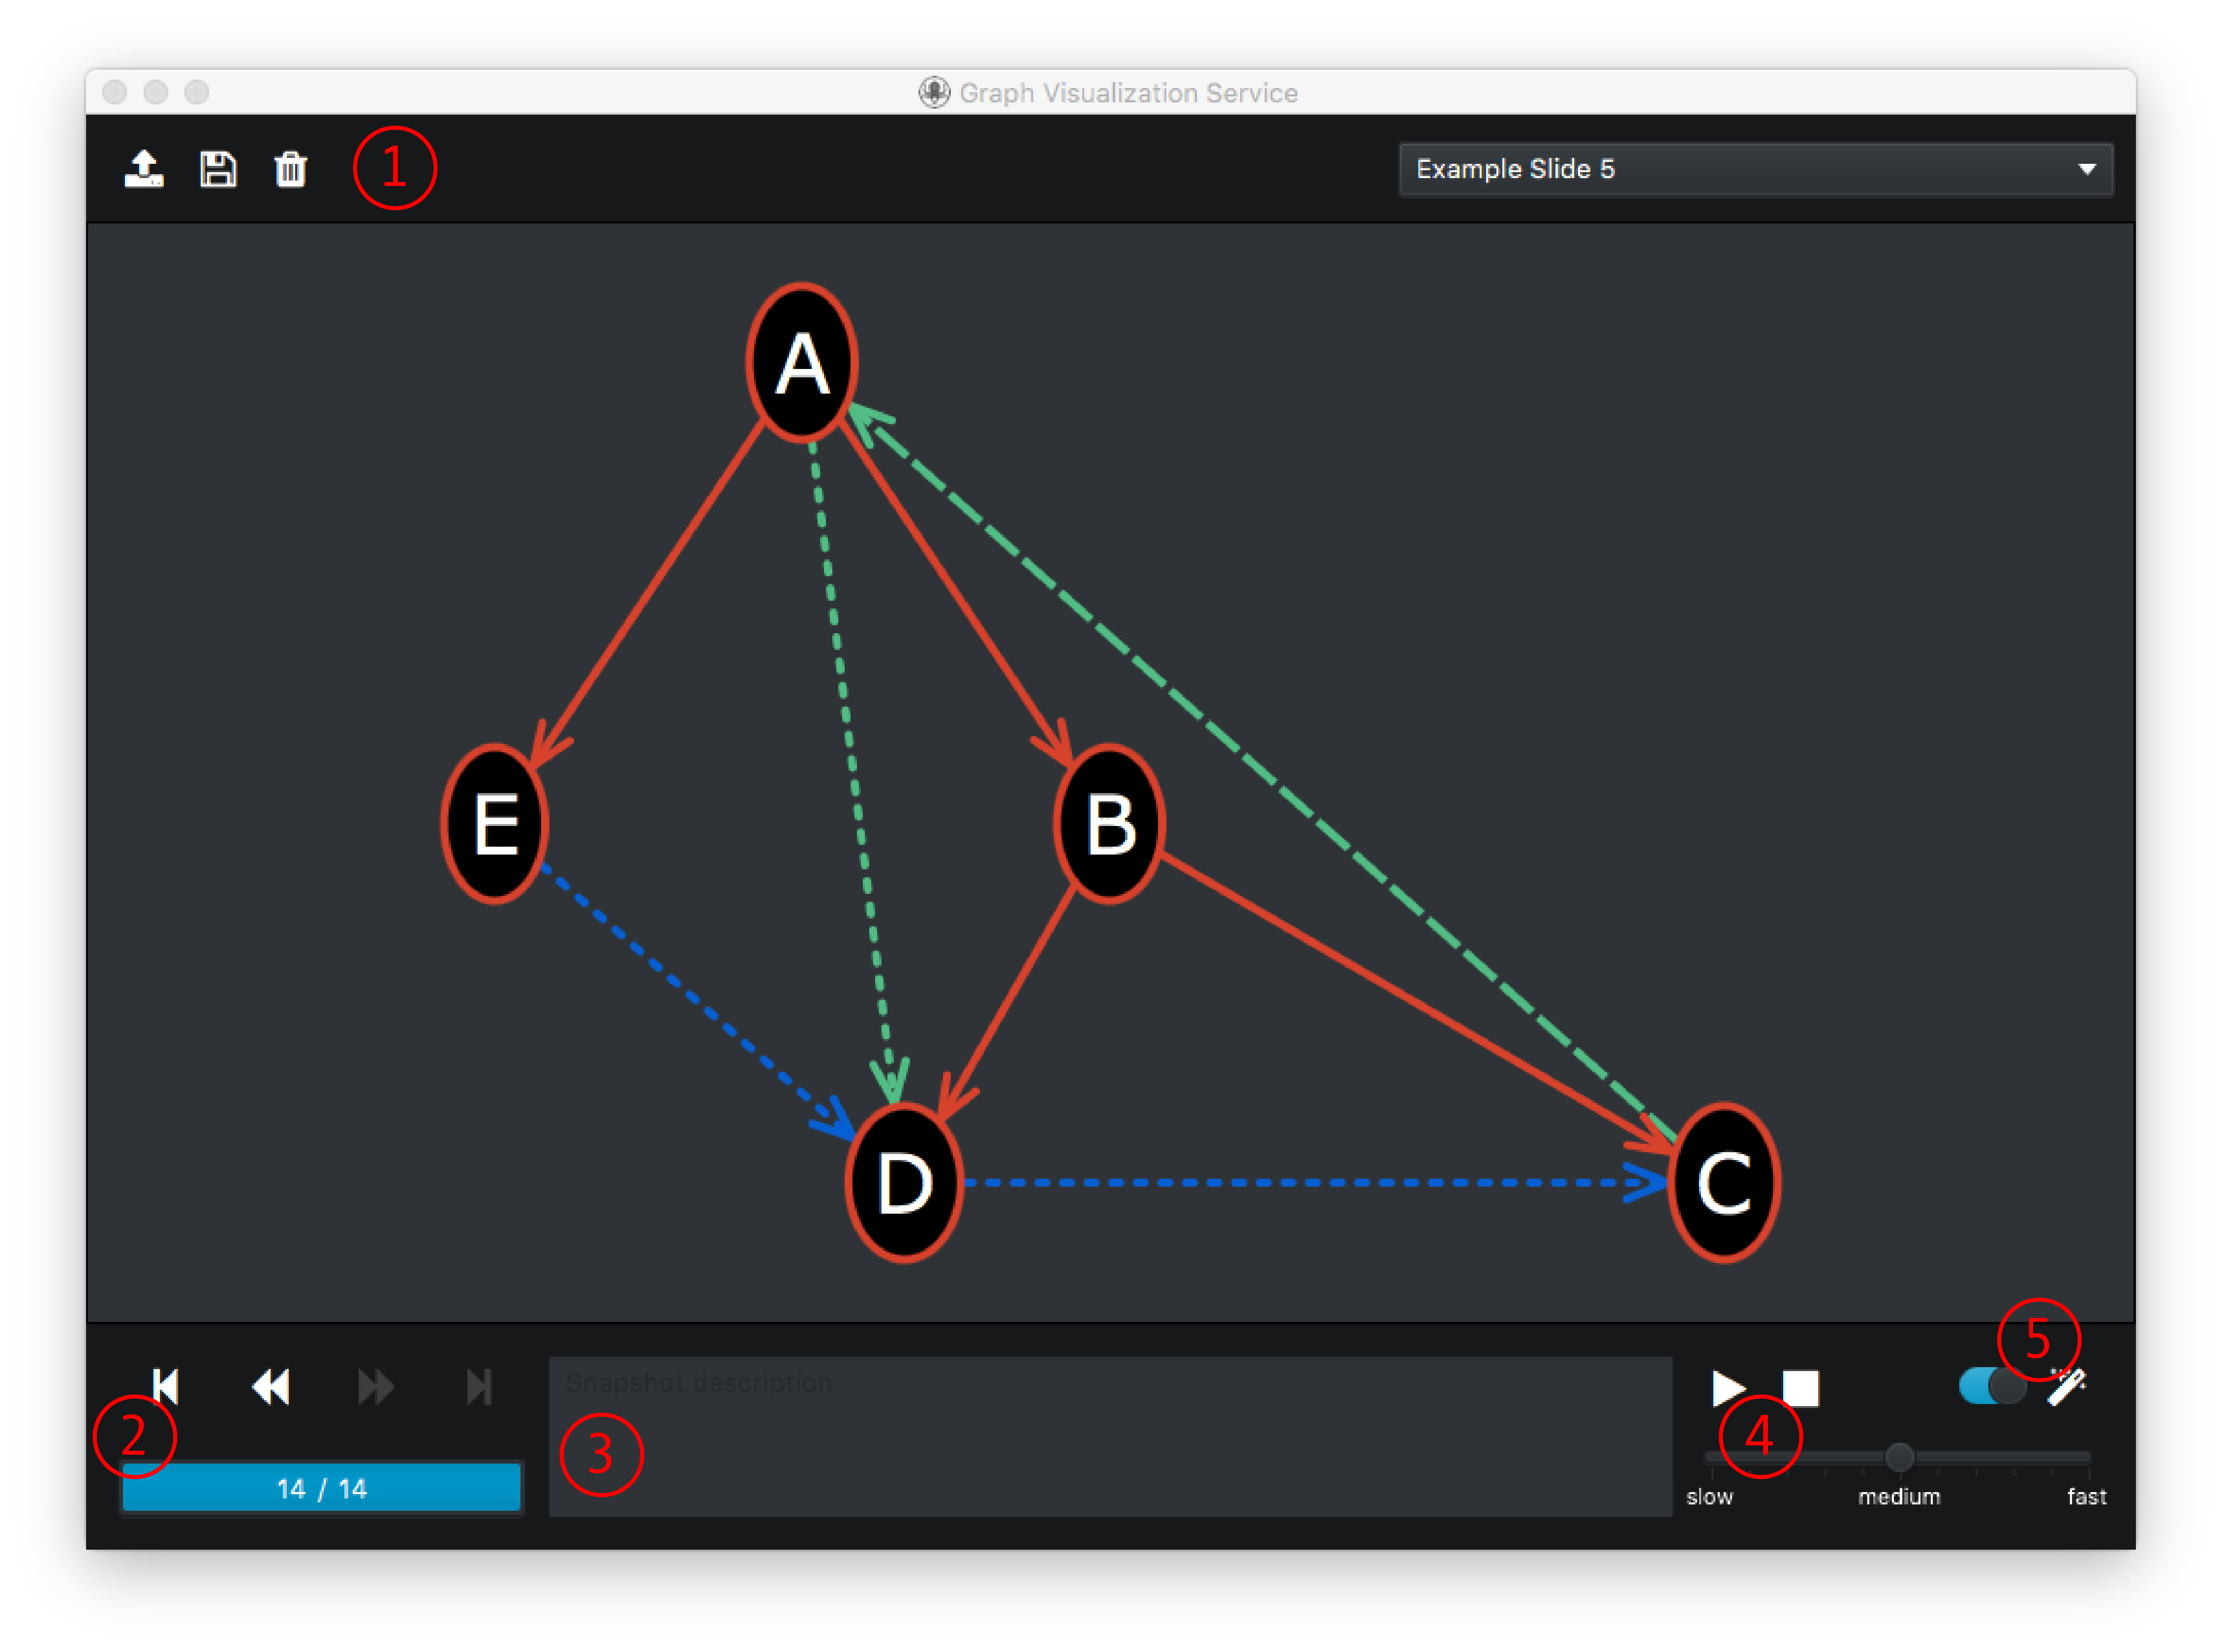
\includegraphics[width=0.7\linewidth]{assets/images/gvs-ui-graph}
		\caption{User Interface GVS 2.0}
		\label{fig:gvs-ui-graph}
	\end{figure}
	
	\subsubsection{1. Toolbar}
	Über die Toolbar, die am oberen Fensterrand dargestellt wird, sind die grundlegenden Aktionen schnell und einfach zugänglich. So kann ein Benutzer eine gespeicherte Session vom Dateisystem laden, die aktuelle Session speichern oder löschen und zwischen den aktuellen Sessions aus der Dropdown-Box wechseln. 
	
	\subsubsection{2. Step Buttons und Fortschrittsanzeige}
	Die Step Buttons bilden zusammen mit der Replay Funktionalität ein wichtiges Werkzeug, um die Funktionsweise eines Algorithmus schrittweise zu analysieren und zu verstehen. Über die Buttons können die einzelnen Momentaufnahmen einer Session durchgeschaut werden.
	
	\subsubsection{3. Snapshot Description}
	Zur aktuellen Momentaufnahme können Notizen erfasst werden. Beim Speichern der Session werden diese ebenfalls gespeichert und werden beim laden der Session wieder angezeigt.
	
	\subsubsection{4. Replay}
	Die Replay Funktionalität automatisiert die Aktionen der Step Buttons in einer bestimmten Geschwindigkeit. Standardmässig wird jede Sekunde zur nächsten Momentaufnahme gewechselt. Das Replay kann nach belieben gestoppt, gestartet und abgebrochen werden.
	
	\subsubsection{5. Autolayout}
	Das Autolayout steht nur für Graphen zur Verfügung. Alle Vertices die noch nicht mit der Maus positioniert wurden, werden vom Graph Layouter so positioniert, dass es möglichst wenig Überschneidungen der Edges gibt. Standardmässig verwendet der Graph Layouter immer zufällige Startkoordinaten. Dies kann über den ToggleButton deaktiviert werden, damit immer das gleiche Layout resultiert.
	
	\subsection{Drag Support}
	Bei Graphen können alle Vertices beliebig mit der Maus positioniert werden. Sobald alle Vertices manuell positioniert wurden, ist die Autolayout Funktion nicht mehr verfügbar. Trees können nicht manuell positioniert werden. Eine entsprechende Meldung wird angezeigt.
	
	\subsection{Zoom Pane}
	Die Zeichenfläche auf der die Graphen und Trees gezeichnet werden, wird automatisch gezoomt und zentriert. 
\end{document}

